%%%%%%%%%%%%%%%%%%%%%%%%%%%%%%%%%%%%%%%%%
% Short Sectioned Assignment
% LaTeX Template
% Version 1.0 (5/5/12)
%
% This template has been downloaded from:
% http://www.LaTeXTemplates.com
%
% Original author:
% Frits Wenneker (http://www.howtotex.com)
%
% License:
% CC BY-NC-SA 3.0 (http://creativecommons.org/licenses/by-nc-sa/3.0/)
%
%%%%%%%%%%%%%%%%%%%%%%%%%%%%%%%%%%%%%%%%%

%----------------------------------------------------------------------------------------
%	PACKAGES AND OTHER DOCUMENT CONFIGURATIONS
%----------------------------------------------------------------------------------------

\documentclass[paper=a4, fontsize=11pt]{scrartcl} % A4 paper and 11pt font size

\usepackage[T1]{fontenc} % Use 8-bit encoding that has 256 glyphs
\usepackage{fourier} % Use the Adobe Utopia font for the document - comment this line to return to the LaTeX default
\usepackage[english]{babel} % English language/hyphenation
\usepackage{amsmath,amsfonts,amsthm} % Math packages

\usepackage{lipsum} % Used for inserting dummy 'Lorem ipsum' text into the template

\usepackage{sectsty} % Allows customizing section commands
\allsectionsfont{\centering \normalfont\scshape} % Make all sections centered, the default font and small caps

\usepackage{lastpage}
\usepackage{fancyhdr} % Custom headers and footers
\pagestyle{fancyplain} % Makes all pages in the document conform to the custom headers and footers
\fancyhead{} % No page header - if you want one, create it in the same way as the footers below
\fancyfoot[L]{} % Empty left footer
\fancyfoot[C]{} % Empty center footer
\fancyfoot[C]{\thepage~of~\pageref{LastPage}} % Page numbering for right footer
\renewcommand{\headrulewidth}{0pt} % Remove header underlines
\renewcommand{\footrulewidth}{0pt} % Remove footer underlines
\setlength{\headheight}{13.6pt} % Customize the height of the header

\setlength\parindent{0pt} % Removes all indentation from paragraphs - comment this line for an assignment with lots of text

%----------------------------------------------------------------------------------------
%	TITLE SECTION
%----------------------------------------------------------------------------------------

\newcommand{\horrule}[1]{\rule{\linewidth}{#1}} % Create horizontal rule command with 1 argument of height



\usepackage{float}

\title{	
\normalfont \normalsize 
\textsc{Norwegian University of Science and Technology\\TDT4136 -- Introduction to Artificial Intelligence} \\ [25pt]
\horrule{0.5pt} \\[0.4cm]
\huge Assignment 3:\\ Using the A* Algorithm\\
\horrule{2pt} \\[0.5cm]
}

\author{Per Magnus Veierland\\permve@stud.ntnu.no}

\date{\normalsize\today}

\newacro{BFS}{Breadth First Search}

\newcommand{\showboard}[4]{
    \begin{figure}[H]
    \centering
    \includegraphics[width=#4\textwidth]{images/#1-#2}
    \caption{#3}
    \end{figure}
}

\newcommand{\showbfs}[2]{\showboard{#1}{breadth_first}{Breadth First Search}{#2}}
\newcommand{\showdijkstra}[2]{\showboard{#1}{dijkstra}{Dijkstra's Algorithm}{#2}}
\newcommand{\showastar}[2]{\showboard{#1}{astar}{A* Search}{#2}}
\newcommand{\showboards}[2]{\showbfs{#1}{#2}\showdijkstra{#1}{#2}\showastar{#1}{#2}}

\hyphenation{Dijkstra}

\begin{document}

\maketitle

\section*{Problem A: Pathfinding in 2D Games}

The \texttt{a1.py} program visualizes A* search in boards with uniform costs and obstacles for A.1.2. The \texttt{a2.py} program visualizes A* search for boards with different costs for A.2.2. The programs \texttt{a3-a.py} and \texttt{a3-b.py} visualizes search using \texttt{BFS}, Dijkstra's algorithm, and A* search for boards with uniform and non-uniform costs respectively for A.3.2. All programs uses the \texttt{vi} Python library which was developed for the IT3105 module.

\begin{figure}[H]
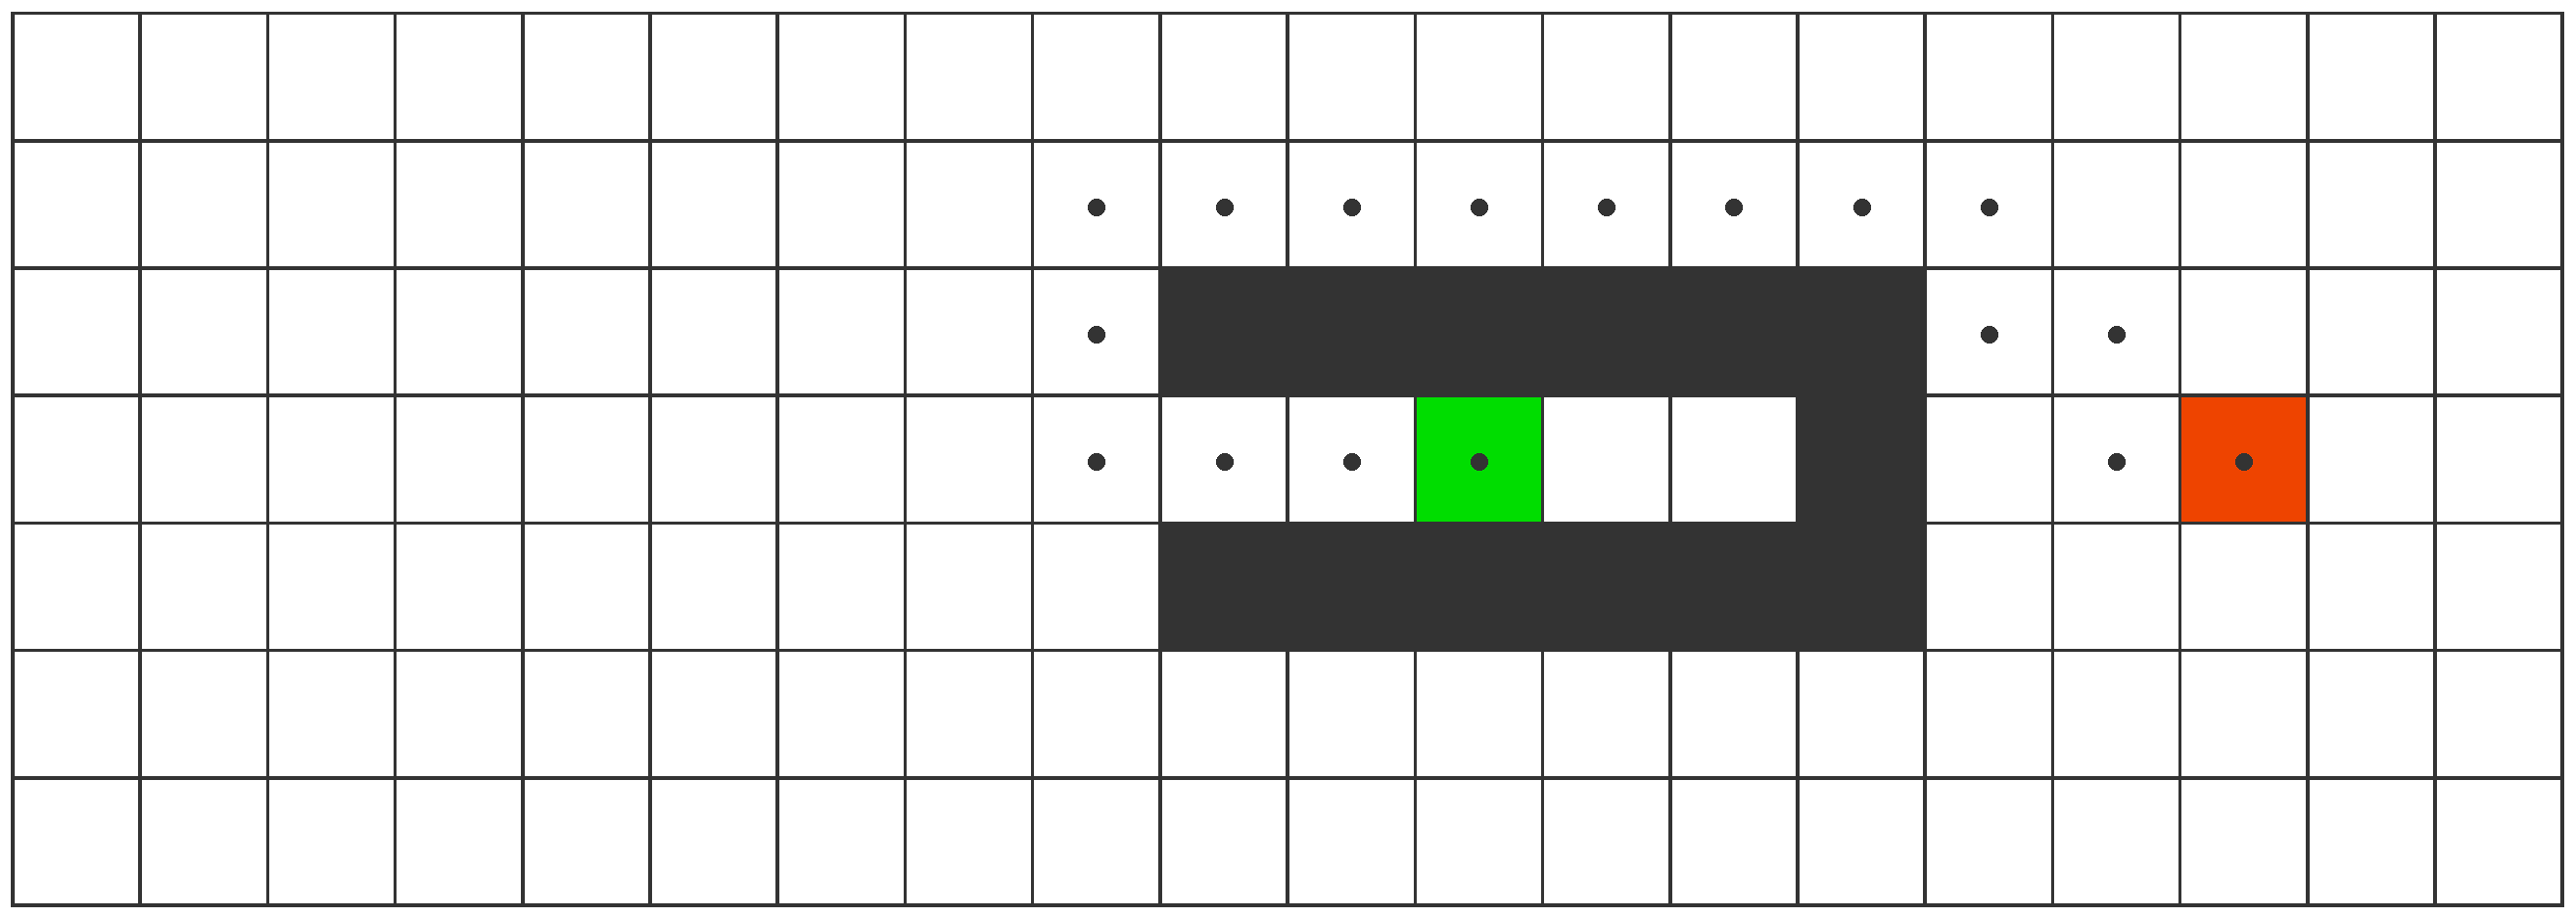
\includegraphics[width=\textwidth]{images/board-1-1}
\caption{\texttt{~board-1-1.txt~}(A* search)}
\end{figure}

\begin{figure}[H]
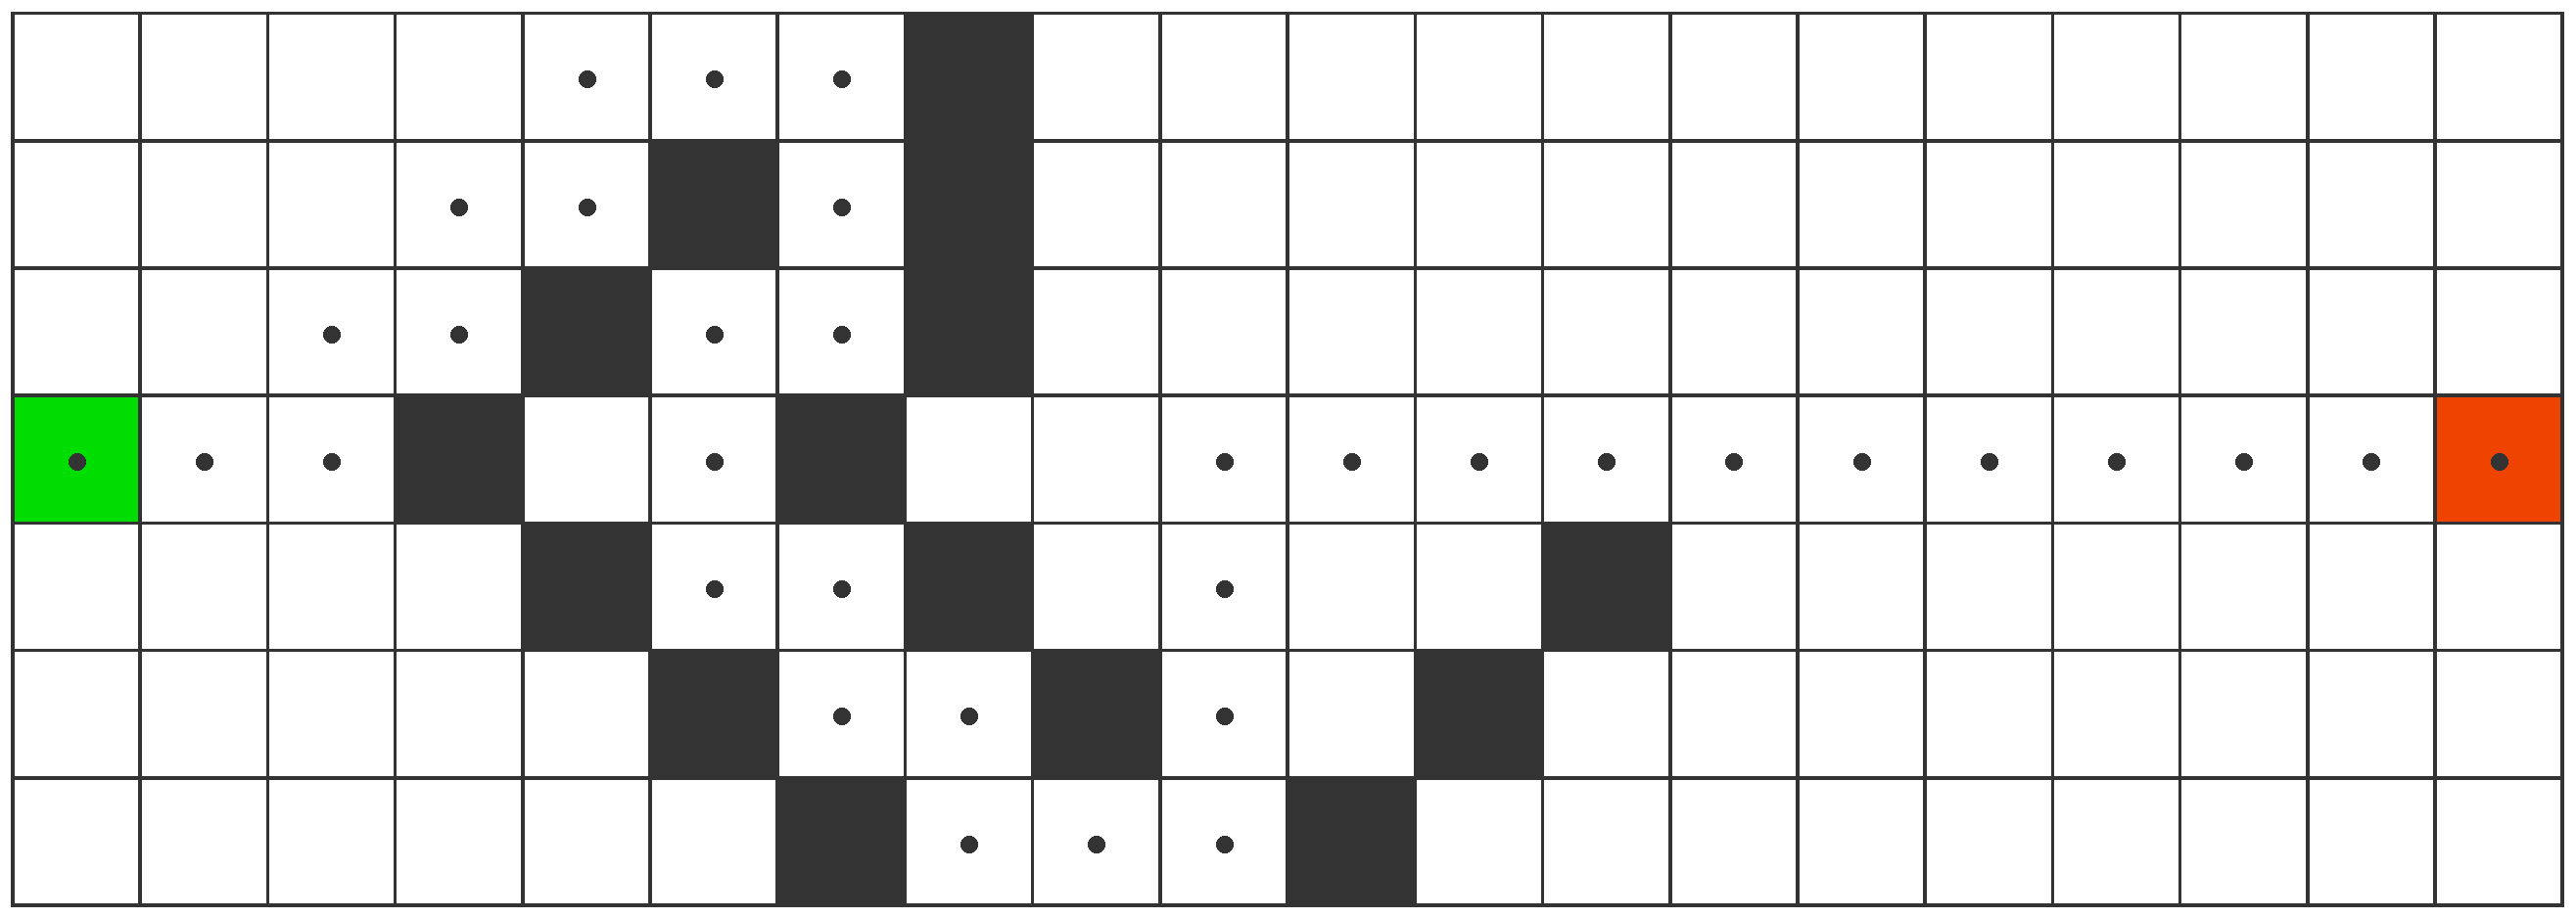
\includegraphics[width=\textwidth]{images/board-1-2}
\caption{\texttt{~board-1-2.txt~}(A* search)}
\end{figure}

\begin{figure}[H]
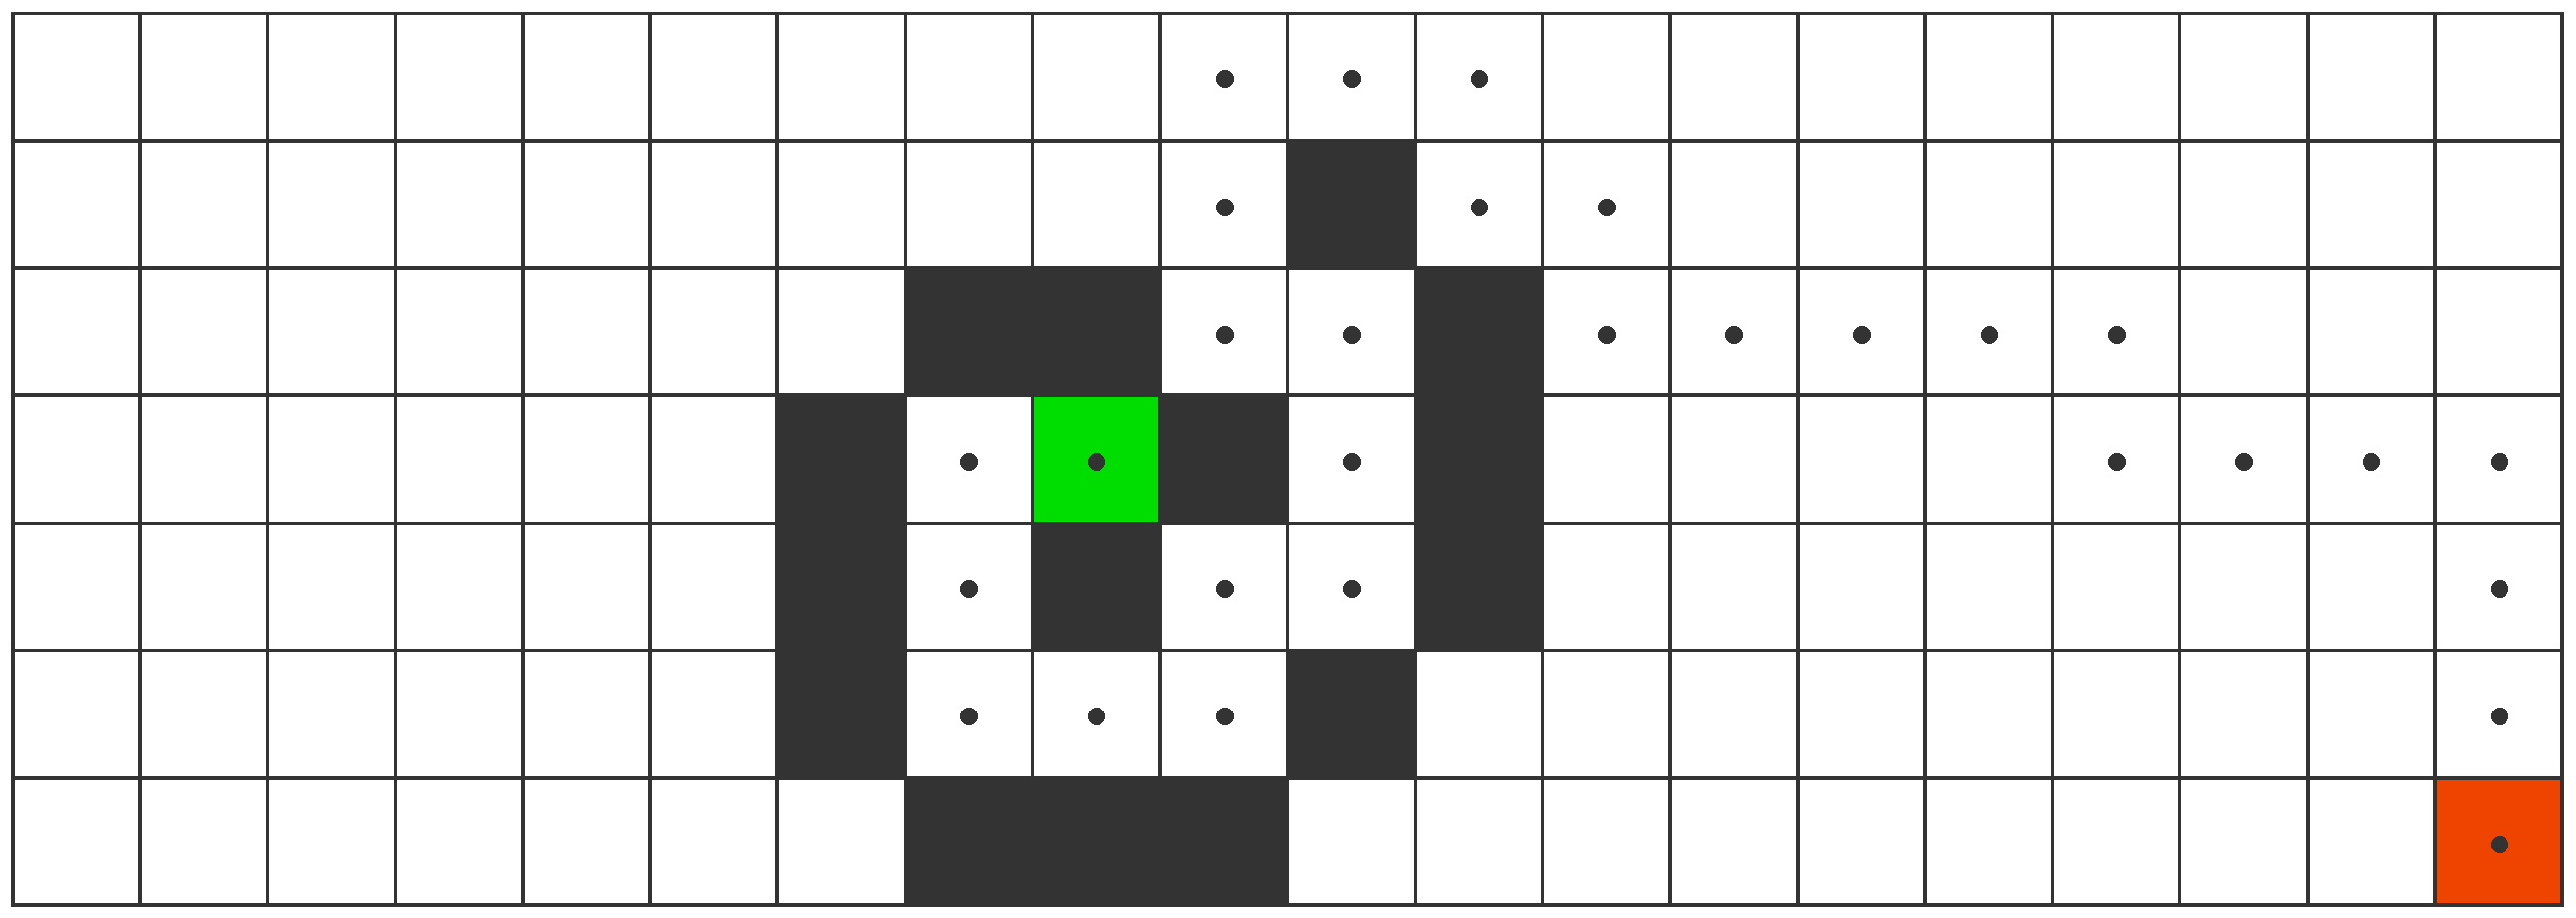
\includegraphics[width=\textwidth]{images/board-1-3}
\caption{\texttt{~board-1-3.txt~}(A* search)}
\end{figure}

\begin{figure}[H]
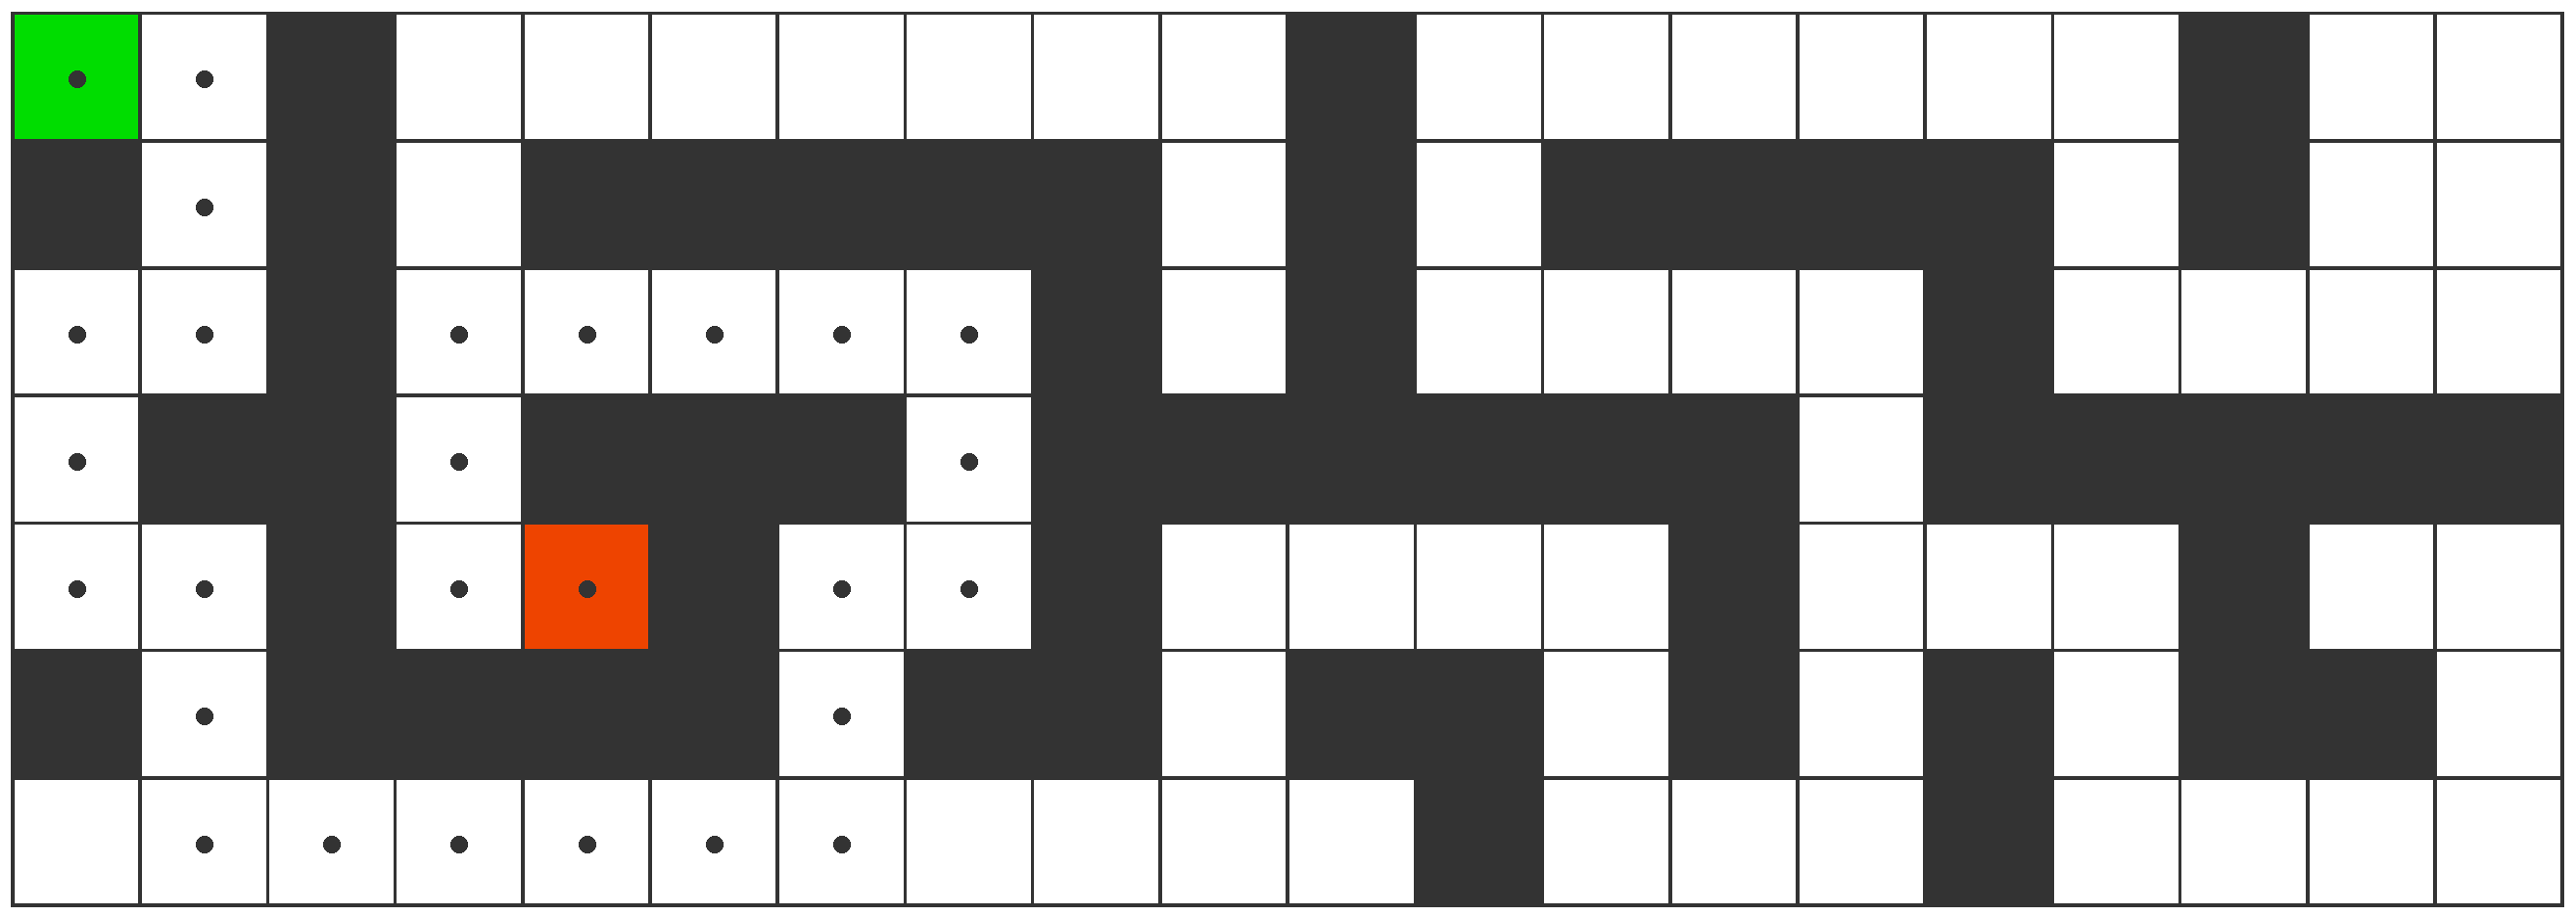
\includegraphics[width=\textwidth]{images/board-1-4}
\caption{\texttt{~board-1-4.txt~}(A* search)}
\end{figure}

\newpage

\begin{figure}[H]
\centering
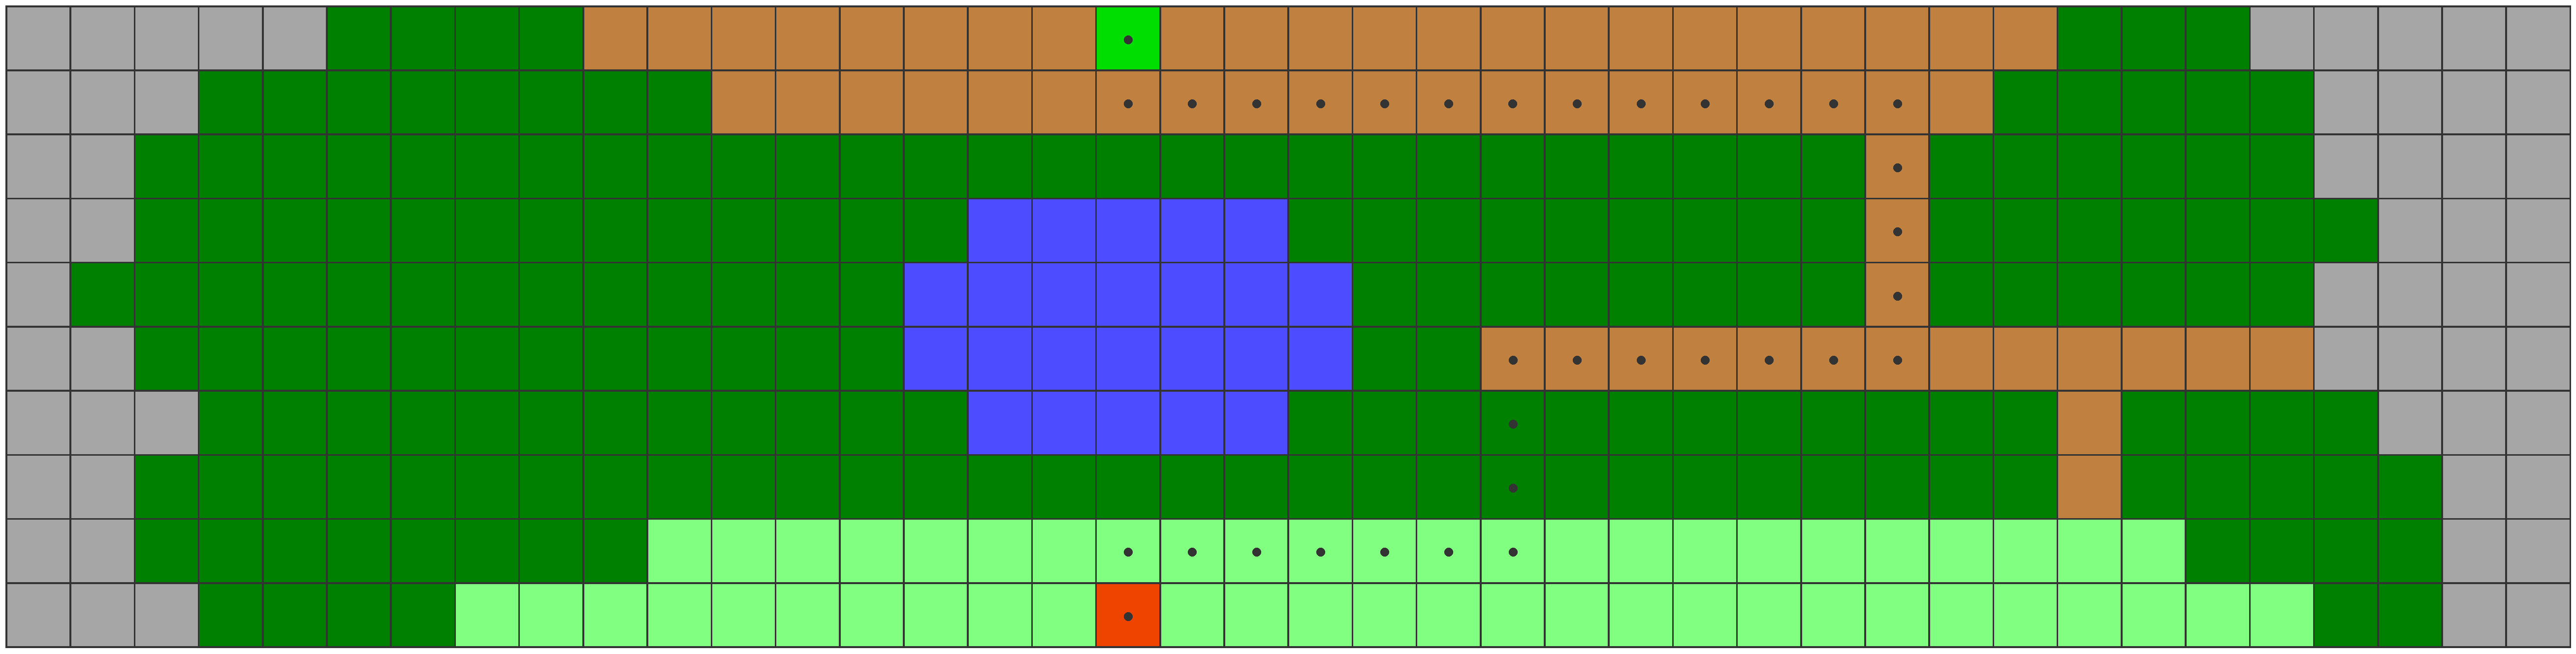
\includegraphics[width=0.9\textwidth]{images/board-2-1}
\caption{\texttt{~board-2-1.txt~}(A* search)}
\end{figure}

\begin{figure}[H]
\centering
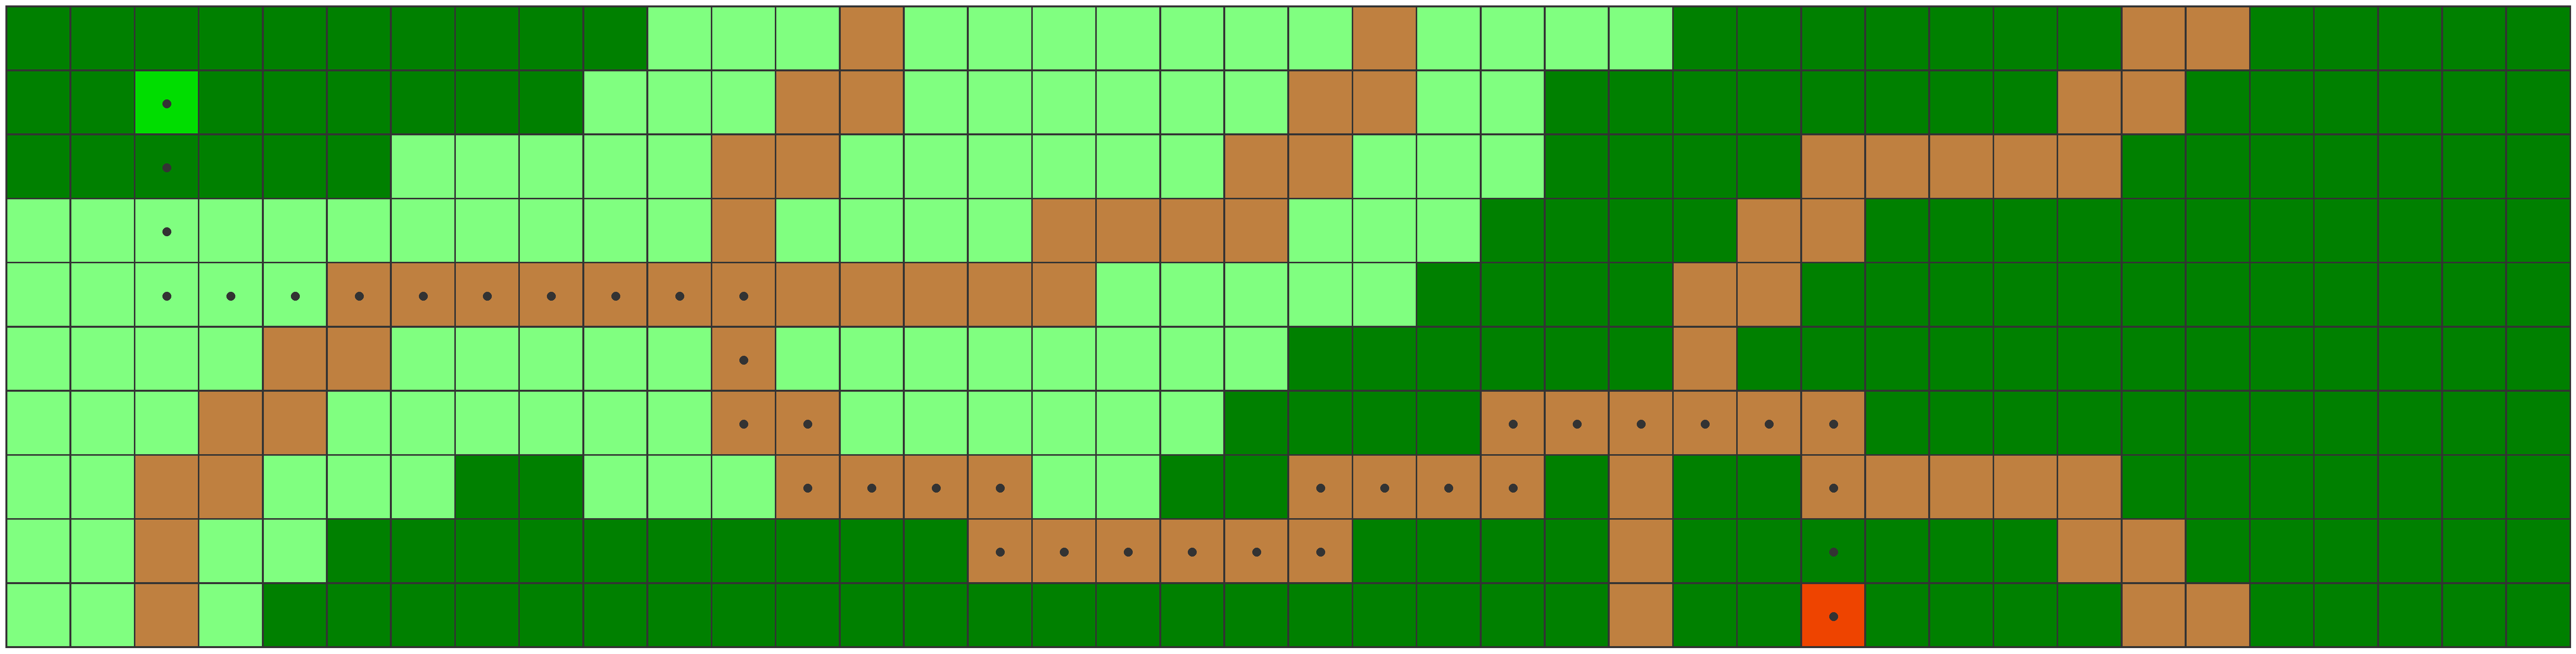
\includegraphics[width=0.9\textwidth]{images/board-2-2}
\caption{\texttt{~board-2-2.txt~}(A* search)}
\end{figure}

\begin{figure}[H]
\centering
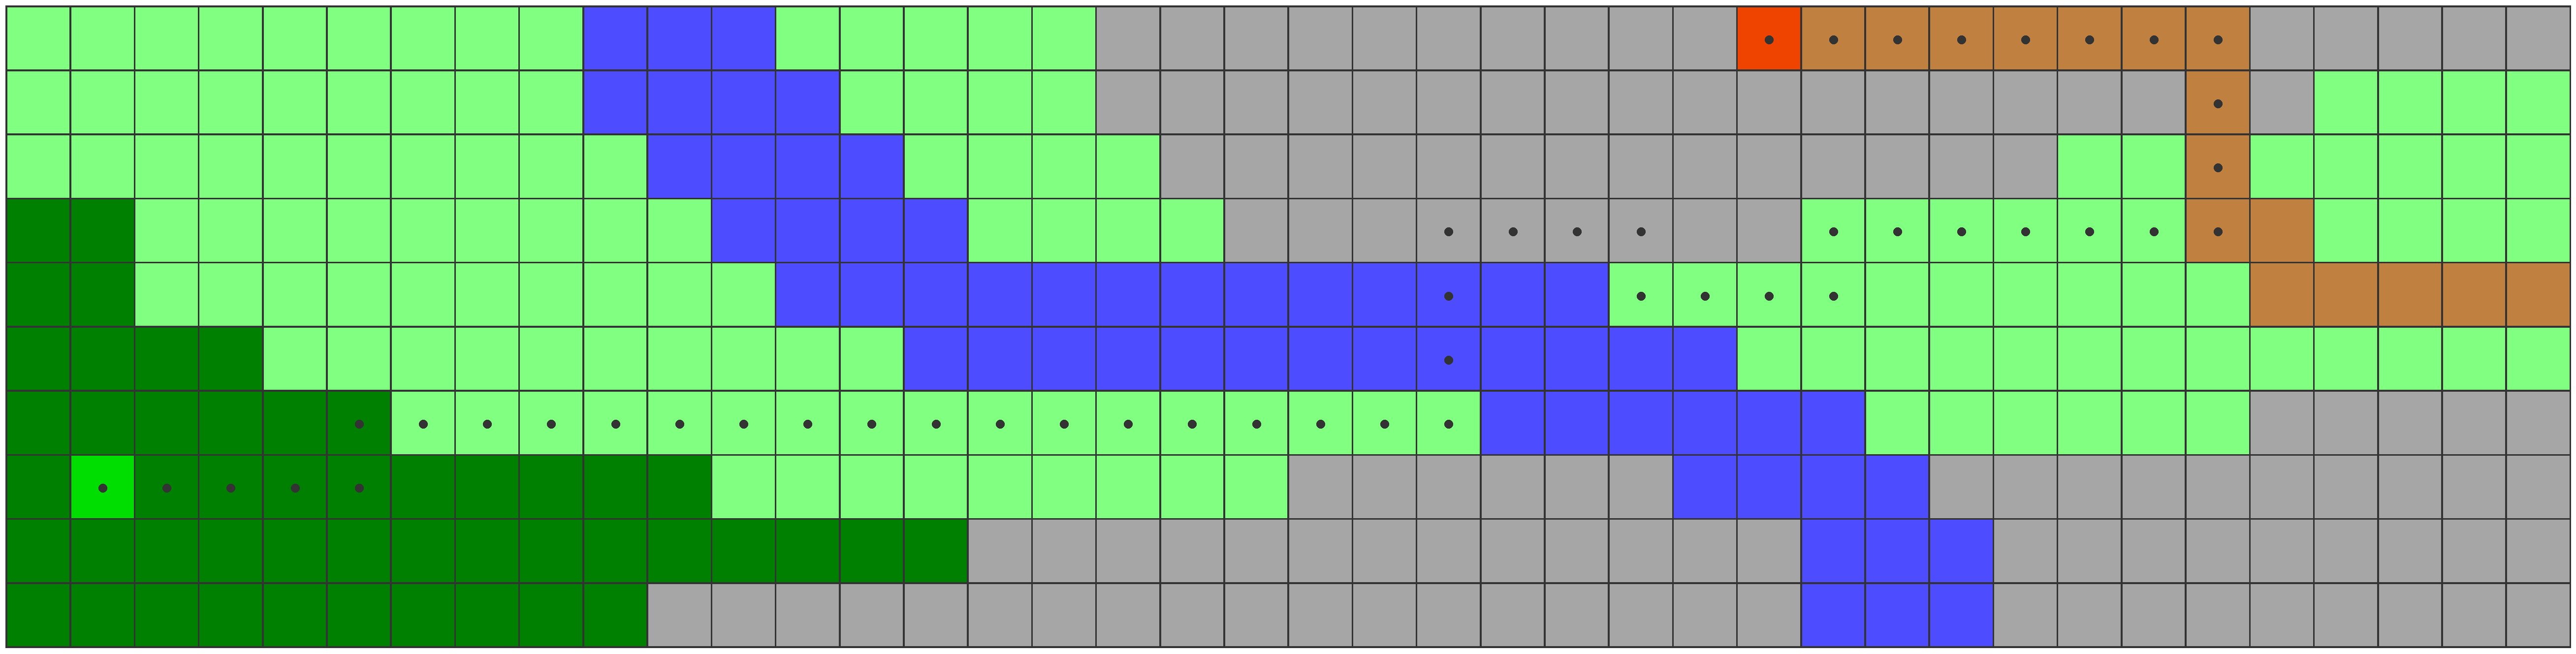
\includegraphics[width=0.9\textwidth]{images/board-2-3}
\caption{\texttt{~board-2-3.txt~}(A* search)}
\end{figure}

\begin{figure}[H]
\centering
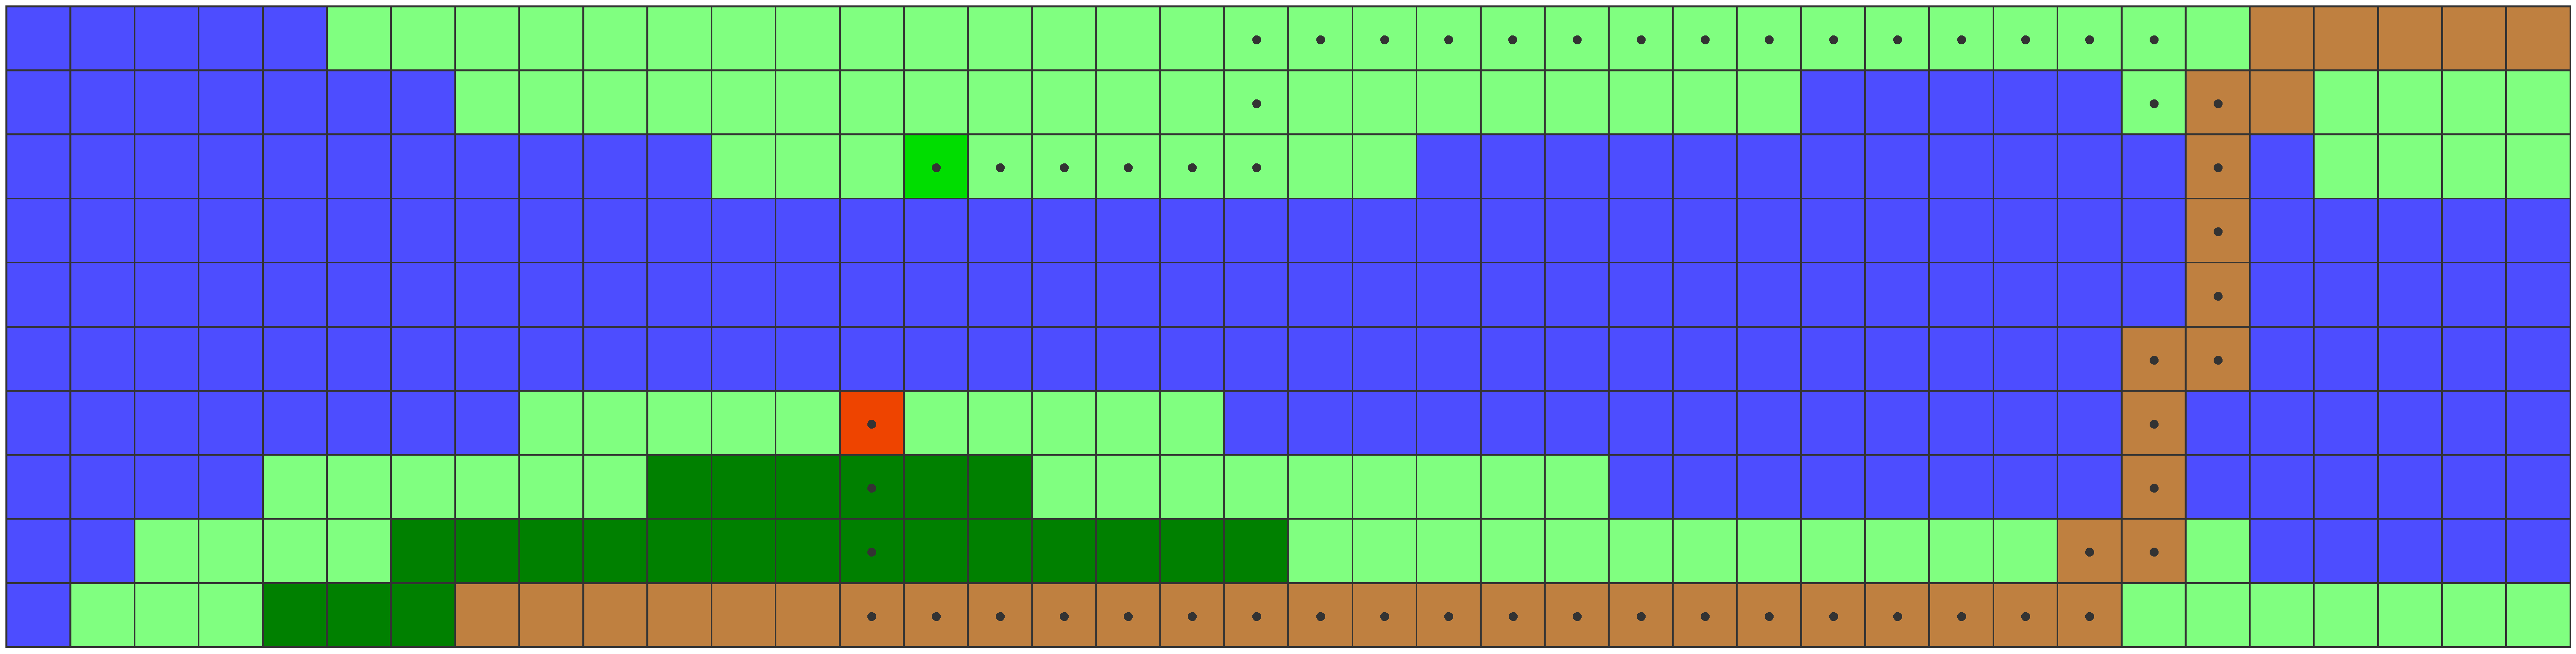
\includegraphics[width=0.9\textwidth]{images/board-2-4}
\caption{\texttt{~board-2-4.txt~}(A* search)}
\end{figure}

\newpage
\subsection*{4.3.3 -- Board-1-1}

Both \ac{BFS} and Dijkstra consider a large number of states and perform almost identically. The A* strategy considers significantly fewer states, but evaluates both symmetrical possible paths to the goal. All three strategies produce optimal paths.

\showboards{board-1-1}{0.75}

\newpage
\subsection*{4.3.3 -- Board-1-2}

Both \ac{BFS} and Dijkstra consider a large number of states and perform almost identically. The A* strategy considers all nodes before the obstacle; but after exiting the obstacle it moves in a straight line towards the goal due to its heuristic. All three strategies produce optimal paths.

\showboards{board-1-2}{0.75}

\newpage
\subsection*{4.3.3 -- Board-1-3}

Both \ac{BFS} and Dijkstra consider all states in the grid. The A* strategy considers significantly fewer nodes and none after the center obstacle. Gaps of states on the ``open list'' in the right grid area can be seen for A* due to its Manhattan heuristic. All three strategies produce optimal paths.

\showboards{board-1-3}{0.75}

\newpage
\subsection*{4.3.3 -- Board-1-4}

It can be seen than \ac{BFS} and Dijkstra consider the same number of nodes; and that they continue the searches in non-goal directions further than A*. All three strategies produce optimal paths.

\showboards{board-1-4}{0.75}

\newpage
\subsection*{4.3.3 -- Board-2-1}

When boards with non-uniform costs are introduced; the difference between \ac{BFS} and Dijkstra's algorithm becomes clear. \ac{BFS} follows all states outwards from the start and ignores costs. It finds the straight path to the goal; however this path is sub-optimal since costs are not uniform. Both Dijkstra and A* finds optimal paths; however A* considers slightly fewer states.

\showboards{board-2-1}{1}

\newpage
\subsection*{4.3.3 -- Board-2-2}

The \ac{BFS} search chooses a straight path which ignores path costs and ends up being quite suboptimal. Both Dijkstra's algorithm and A* search finds the optimal paths; but Dijkstra's algorithm considers a few more states than A* due to its lack of a heuristic.

\showboards{board-2-2}{1}

\newpage
\subsection*{4.3.3 -- Board-2-3}

The \ac{BFS} appears to do well in this scenario and finds a path close to the optimal. However it still traverses more water cells and mountain cells than the optimal path. Both Dijkstra's algorithm and A* search finds the optimal paths; but Dijkstra's algorithm considers a few more states than A* due to its lack of a heuristic.

\showboards{board-2-3}{1}

\newpage
\subsection*{4.3.3 -- Board-2-4}

The \ac{BFS} search traverses states equally in all directions and finds the path to the goal which is the fewest number of states away; but which has a much greater path cost than the optimal path. Both Dijkstra's algorithm and A* search finds the optimal paths; but Dijkstra's algorithm considers a few more states than A* due to its lack of a heuristic.

\showboards{board-2-4}{1}

\end{document}

